

\begin{figure}
    \centering
    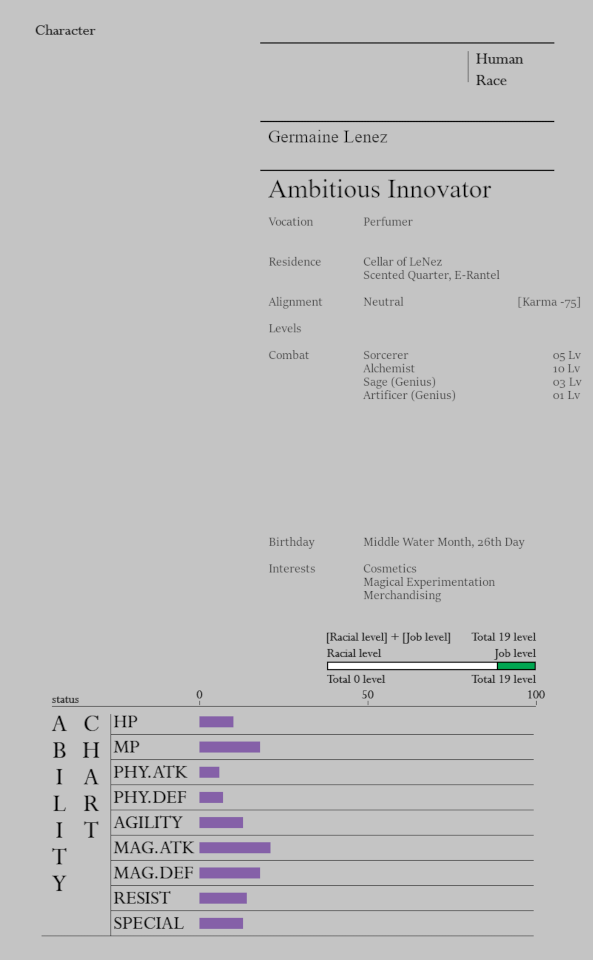
\includegraphics[width=1\linewidth]{V1 Birthright//images/ucThEId.png}
    \caption*{Germaine Lenez Character Sheet}
\end{figure}

\section*{Arcane Artisans}

Not all of those who are gifted with aptitude for the arcane become mages who seek their fortune as Adventurers, nor do they join the ranks of the armies or noble retinues of their nation. Neither do they become magisters that walk erudite halls to instruct on and delve into the great mysteries of the art.

 

Indeed, a great many mages do not even spare a thought to the vocations that may place them in mortal danger, or those of study for its own sake. They do not seek an Adventurer’s fame or the grand campaigns of mighty armies; nor the company of their fellows in seclusion from the unlearned and ignorant masses of the world.

 

Instead, they turn their considerable skills towards the production of goods and services for towns and cities, selling their wares to noble patrons and common labourers alike. No simple apothecary or dabbler in enchantment and artifice can match the expertise and quality of those who endeavour to become masters of their respective crafts.

 

From lifesaving potions and magical equipment to enchanted tools that improve the quality of daily life and labour, these artisans form one of the cornerstones of civilized societies around the world. Their endless quest for its improvement makes them integral to development beyond simple agrarian life, and their work often comes hand in hand with the rise of advanced and powerful nations.

 

Though their focus may lie in serving on the industrial side of civilian settings, they are still potent arcane casters that often wield the same spells as one would find used by an Adventurer or Military Mage, as their research leads them to seek out answers in every field of magic available to them. Many an ignorant belligerent or nosy official have found themselves burned, electrocuted, frozen or melted – even transmuted into useful materials by an incensed shopkeeper to exact payment for the disruption of their business.


\chapter{Ludmila Zahradnik}

Ludmila and Lady Shalltear rested on a bench placed in the shade of a tree that had been left to grow off the street near the Perfumer’s shop. The Vampire was idly staring at the clear afternoon sky while Ludmila was once again busy recalculating her once again obsolete budget.

 

“You seem to be taking this all in stride,” Lady Shalltear spoke as she watched the wisps of the remaining clouds drift away as they journeyed southwards.

 

“My head is still spinning from all this, actually,” Ludmila said. “Ninety-six platinum is a lot of money, is it not, my lady?”

 

“I wouldn’t know,” Lady Shalltear said. “I’m no more aware of the value of anything than I was an hour ago.”

 

“I’m sorry, my lady,” Ludmila apologized. “My mind is swamped just trying to keep up with everything. Ninety-six platinum is enough to feed, clothe and arm every villager in Warden’s Vale for an entire year. Or at least it would be, if they were still around.”

 

“Well, if you put it that way, it seems like it would be a significant sum for one of you…but you made it sound as if your territory is small; is this not the case?”

 

“It is,” Ludmila nodded. “There were only thirty households last summer.”

 

“And how does that compare to the other nobles?” Lady Shalltear asked.

 

“Corelyn Barony has around two thousand households, last I heard,” Ludmila dredged up the numbers from her memory. “Countess Jezne should have close to five thousand households in her personal demesne alone. Then there are five other baronies within her territory, but they aren't as productive as the Riverlands, so perhaps double that in the whole of Jezne County.”

 

She frowned and made a vexed noise.

 

“I guess once I actually look at the numbers from that perspective, it’s not so much. Ninety-six platinum would barely last two days if Countess Jezne suddenly had all of her production cease like it has right now. I suppose this is what most people see when they look at the nobility and their revenues: they think about what they would personally purchase for themselves if they had access to such wealth, with no obligations. Ninety-six platinum coins for an average city labourer is over twenty-five years of work.”

 

“Your demesne is vacant now,” Lady Shalltear said. “It seems like you do indeed have that much for yourself.”

 

“It belongs to House Zahradnik,” Ludmila stated. “The revenues of the demesne should go towards its development and growth for greater gains in the future. After hiring and providing for the manor household, purchasing the tools and other supplies for the labour force, and buying what is needed to maintain the village, I will still have the majority of this capital to work with. I need to see about attracting new tenants and investing in services and industries for the village to support the surrounding lands as they are developed.”

 

“You seem to have a clear picture concerning the future of your territory.”

 

“The frontier territories are far behind in development compared to the interior regions,” Ludmila said. “There is much to study and learn from what the other nobles have done. But what works for them may not necessarily work for me – I have a few ideas but, by and large, it will just be a lot of trial and error: which I suspect is where most of my capital will vanish.”

 

“For someone with such a progressive outlook,” Lady Shalltear said, “that sounded quite pessimistic.”

 

“I did not mean for it to sound that way, my lady, but after looking at the filled-out parts of the almanacs that the administration provided…if they are accurate, then the nobility cannot rely on their past to model the future.”

 

Seeing Lady Shalltear’s face turn blank in confusion, Ludmila realized how cryptic her last sentence sounded.

 

“It’s the Undead workforce, my lady,” she explained. “If the Sorcerous Kingdom can field this labour in quantities enough to fill the needs of every territory, then our economies are fundamentally changed. For a fraction of the cost of providing for tenant farmers, these Undead servitors can do the same work. The same goes for any other sort of menial labour that they can manage. That means we will need far fewer tenants working directly as labourers, and more tenants that are capable of directing the Undead in tasks that benefit from specialized direction.

 

The nature of value will shift drastically – any goods produced with the assistance of Undead labour will become cheaper relative to those produced by more complex tasks that still require the expertise of skilled craftsmen. Territories that have vast amounts of arable land will be able to thrive through sheer volume of agriculture, but those that do not will need to find or create something unique to their own territories that set them apart from the rest. Warden’s Vale falls into the latter category: for the time being I can rely on forestry and the limited agricultural space we have, but the terrain of the highlands makes development like you see in the interior difficult and expensive by comparison.”

 

Ludmila looked around at the empty street, continuing to share her thoughts with Lady Shalltear.

 

“The entire region will feel these changes, I think. E-Rantel is the hub of inland trade between Re-Estize, the Empire and the Theocracy. I’ve seen those that look like they come from places even further out as well. Once the duchy comes back to life and commerce resumes, the city will be swarmed with traders who will seize the opportunity to buy the goods that the Sorcerous Kingdom produces at significantly lower costs.”

 

“I think you’ve gotten so used to us that you forget that most people are rather averse to the Undead,” Lady Shalltear said.

 

“You are correct, my lady,” Ludmila conceded, “but, like this city, it should only be a matter of time. The most intrepid merchants will carry the Sorcerous Kingdom’s products far and wide, and their guildmates will see their caravans laden with commodities obtained at prices impossible elsewhere. Ambition will overcome fear – the only fear will be the fear of falling behind their rivals and competitors, and that will drive them all the more.”

 

“So...how long would you say until this happens?” Lady Shalltear leaned towards her, “This vision you conjure seems to fulfill a part of His Majesty’s wishes.”

 

“If trade is allowed to flow freely, a few years, perhaps,” Ludmila said. “Not more than a decade for the immediate region. The only obstacles that come to mind would be the political and cultural barriers that may form in opposition to the growing power of the nation – or the nature of the Sorcerous Kingdom itself. Since the Undead will be doing most of the menial labour, someone might spread rumors of cursed foodstuffs, for instance.”

 

“Those Skeletons are incapable of casting curses,” Lady Shalltear muttered. “We should find the individuals that spread these baseless rumors and silence them.”

 

“That is a needless effort which may cause more problems than it solves, my lady; it can be safely ignored, I think. Merchants will find ways around those barriers to facilitate trade, and even a formal trade embargo seems self-defeating. Over time, those that embrace our nation’s trade will thrive compared to those that do not due to the cost of our goods. If nations do not yield to this trade, they will slowly lose ground to their rivals until their lands are forcefully taken from them. So, sooner or later, they will fall under the Sorcerous Kingdom’s economic hegemony. If they wage war to break the hegemony, they will only provide the justification to be crushed by His Majesty’s armies.”

 

“Did you realize this all on your own, while sitting on this bench?” Lady Shalltear examined the rough wooden construction of their seat suspiciously.

 

“It is the knowledge and experiences of the past day coming together…and perhaps I have been raised in part to see things from this perspective for my entire childhood.” Ludmila’s gaze turned inwards. “Realizing possibilities makes you come into other possibilities. As resources become available and knowledge grows, things that I would not have not conceived of come into view. As each hour passes, my life seems to become busier – I want to see and do more, and the hours of the day seem ever more insufficient. Besides, that should be the reason why the annexation of this duchy came in the form that it did, yes?”

 

“Um...maybe?” Lady Shalltear’s gaze shifted away, “Some of the others should understand at least this much, but even the most intelligent amongst us can only hope to skim the surface of His Majesty’s limitless insight.”

 

“The laws of Re-Estize have been kept intact,” Ludmila stated, “which means that His Majesty has left the management of its territories to those that already have a firm grasp on the characteristics of their respective fiefs. The policies and mechanisms of the administration have been set up so that we can smoothly adopt the concepts that the Royal Court wishes to introduce to the nation so they can, in turn, realize their goals for industry and trade. As all of the pieces fall into place, this grand strategy will become an unstoppable current – one can either have it carry them comfortably to where it brings us, or be swept away forcefully to the same destination regardless.”

 

Lady Shalltear was silently mouthing something as she digested Ludmila’s words. Her expression suddenly sharpened, though, and she turned her head to the south.

 

“Oh, they found something,” she said.

 

“My lady?” Ludmila twisted around to look to the storefront to see if Aemilia had come out.

 

“Not them. The members of my Household that I sent to locate your ship.”

 

“Really, my lady?” Ludmila rose from her seat, “Where did they find it?”

 

“I don’t think I’ve seen a name for it on the maps. There’s a steep section of the valley, where the river goes through a series of large bends. The ship they see has run aground on the bank.”

 

“I know where that is…the shores are rocky though,” Ludmila frowned worriedly, “is there any damage, my lady?”

 

“They can’t tell,” Lady Shalltear replied. “Shall we go take a look?”

 

Ludmila thought for a moment before deciding to wait.

 

“We should wait and return to the house with the wagon, my lady.”

 

“What about the food you still have to sell?” Lady Shalltear asked, “The Merchant Guild as well, to collect your payments.”

 

“Seeing today’s revenues thus far, I can provision the city manor with it instead,” Ludmila answered. “It should be enough to keep the household staff fed for a while without needing to access the city’s limited supplies. We can drop by the Guild after we’ve seen to the vessel.”

 

As they made their way back to the wagon, the front door of the workshop opened. The heat and odours of its interior once again wafted out into the street and Aemilia emerged with a small, lacquered Rosewood chest held in both hands. One of the Vampire Brides was holding a smaller box with a similar appearance. Germaine followed after them, closing the door lightly behind her with a grin on her face.

 

“It looks like they found something for you as well, my lady.” Ludmila noted, but Lady Shalltear only tapped her lip thoughtfully.

 

The Perfumer came up to Ludmila and held up two sheets of high quality paper.

 

“This one’s the bill for what your Lady’s Maid purchased,” Germaine said as she handed over the first, then the second, “and this one’s the invoice for the Merchant Guild. You can move your wagon into the alley where we’ll grab the rest of your things and get those trees into the warehouse.”

 

Ludmila motioned to the Soul Eater to do as Germaine instructed, then looked down to the bill.

 

Aemilia had ordered quite a long list of items. There were two sets of women’s perfume for each member of the household staff – one set for use during functions held during the day, and another for those held during the evening. There were also a dozen vials of cologne for the manservants that would be hired; she wondered if the Undead footmen were expected to use it as well. She scanned over two crates of aromatic candles and one crate of scented soap as her eyes ran down the list to the end, where the items for her personal use were. Three sets of perfume, soaps, candles, bath salts and scents for her solar. She didn’t even know where to start on their use; her experience with fragrances was next to nonexistent, given the remote location of Warden’s Vale and the impracticality of using cosmetics that could easily make Demihumans aware of one’s presence.

 

Her eyes felt like they would roll out of their sockets when she read the tally at the bottom: eighty gold coins – eight platinum coins had disappeared before they had even entered her hands. She looked up with a question on her tongue, but Aemilia’s beaming face seemed so confident and pleased at her selection that Ludmila’s words were left unspoken.

 

“Is there one for me?” Lady Shalltear said as she peeked around Ludmila’s arm at the bill.

 

“Hmm…well that one’s a gift?” The Perfumer replied, “You said you were a Cleric, but if one of the city temples here had someone like you, they’d be overflowing with ‘supplicants’ every day. That means you must be a big shot on the King’s side, right? The Baroness here defers to you, after all. Just let people know what you’re wearing if they ask, and where it comes from. It’ll be great for marketing.”

 

“Lady Shalltear is the Minister of Transportation,” Ludmila informed her.

 

“Ahaha…”

 

Germaine abruptly turned around and quickly walked off after the wagon that had disappeared around the corner and into the alley.

 

Ludmila instructed the Death Knights to help with the cargo, then turned back to Lady Shalltear. She was holding up a clear crystal vial about the length of her pinky finger against the sky, peering at the liquid inside. She suddenly flicked the vial into the air, and it tumbled end over end before falling again to hit the stone pavement at her feet. Rather than shattering, it bounced several times before spinning to a halt. She knelt to pick up the vial again.

 

“The vial has a petty enchantment reinforcing it,” she noted with interest, “and since it has become a magic item, it won’t break without one purposely destroying it. How quaint.”

 

“What did they find for you, my lady?” Ludmila was curious about what the Vampire Brides found that they thought suited their mistress.

 

Lady Shalltear removed the stopper of the vial and turned it over against her wrist. After testing the scent with a focused expression, she extended her arm. Ludmila leaned forward: it was rich and earthy, with the hint of green and dried flowers. The ghost of incense could be detected, so faint that it gave the impression it was not actually there.

 

“A winter meadow? No, it wouldn’t have incense mixed in then,” Ludmila could not quite place the fragrance.

 

“A mausoleum,” Lady Shalltear offered, “or a tomb. The aroma of turned earth, dried flowers and incense in a long forgotten offering to the past.”

 

Her words came together with the fragrance of the perfume to create vivid imagery. Of cold stone in pristine silence; the peace of the grave seducing the weary to rest.

 

“It suits you very well, my lady,” Ludmila agreed with the selection. “Her quirks aside, Germaine is an excellent Perfumer…do you think she would accept an offer to move her workshop to Warden’s Vale? It is much cooler there throughout the year, and she expressed an interest in what could be gathered in the region.”

 

“If you believe so. I can hardly advise you in matters of your own demesne.” Lady Shalltear said, then smirked, “Though you may want to be able to survive an Acid Cone or two first.”

 

The rattling of the now mostly empty freight wagon drew their attention as the Soul Eater drove it back onto the street. Aemilia and the Vampire Brides were already sitting in their usual seat on the rear edge of the wagon. The Death Knights stomped out after them, but Germaine was nowhere to be seen.

 

“Where’s the Perfumer?” Ludmila asked them as she and Lady Shalltear pulled themselves into the front seat.

 

“Miss Lenez stayed behind in her workshop, my lady,” Aemilia answered. “She looked ready to get to work.”

 

“It seems like I will have to make my offer some time later,” Ludmila said, “not that I am in any way ready to accommodate an Alchemist. We are heading back to the manor to drop everything else off. There is something I need to check on before we go out to purchase the rest of what is needed.”